%%%%%%%%%%%%%%%%%%%%%%%%%%%%%%%%%%%%%%%%%%%%%%%%
%% Intro to LaTeX and Template for Homework Assignments
%% Quantitative Methods in Political Science
%% University of Mannheim
%% Fall 2017
%%%%%%%%%%%%%%%%%%%%%%%%%%%%%%%%%%%%%%%%%%%%%%%%

% created by Marcel Neunhoeffer & Sebastian Sternberg


% This template and tutorial will help you to write up your homework. It will also help you to use Latex for other assignments than this course's homework.

%%%%%%%%%%%%%%%%%%%%%%%%%%%%%%%%%%%%%%%%%%%%%%%%
% Before we get started
%%%%%%%%%%%%%%%%%%%%%%%%%%%%%%%%%%%%%%%%%%%%%%%%

% Make an account on overleaf.com and get started. No need to install anything.

%%%%%%%%%%%%%%%%%%%%%%%%%%%%%%%%%%%%%%%%%%%%%%%%
% Or if you want it the nerdy way...
% INSTALL LATEX: Before we can get started you need to install LaTeX on your computer.
				% Windows: http://miktex.org/download
				% Mac:         http://www.tug.org/mactex/mactex-download.html	
				% There a many more different LaTeX editors out there for both operating systems. I use TeXworks because it looks the same on Windows and Mac.
				

% SAVE THE FILE: The first thing you need to do is to save your LaTeX file in a directory as a .tex file. You will not be able to do anything else unless your file is saved. I suggest to save the .tex file in the same folder with your .R script and where you will save your plots from R to. Let's call this file template_homework1.tex and save it in your Week 1 folder.


% COMPILE THE FILE: After setting up your file, using your LaTeX editor (texmaker, texshop), you can compile your document using PDFLaTeX.
	% Compiling your file tells LaTeX to take the code you have written and create a pdf file
	% After compiling your file, in your directory will appear four new files, including a .pdf file. This is your output document.
	% It is good to compile your file regularly so that you can see how your code is translating into your document.
	
	
% ERRORS: If you get an error message, something is wrong in your code. Fix errors before they pile up!
	% As with error messages in R, google the exact error message if you have a question!
%%%%%%%%%%%%%%%%%%%%%%%%%%%%%%%%%%%%%%%%%%%%%%%%


% Now again for everyone...

% COMMANDS: 
	% To do anything in LaTeX, you must use commands
	% Commands tell LaTeX when to start your document, how you want your document to look, and how to format your document
	% Commands ALWAYS begin with a backslash \

% Everything following the % sign is a comment and will not be used by Latex to compile your document.
% This is very similar to # comments in R.

% Every .tex file usually consists of four parts.
% 1. Document Class
% 2. Packages
% 3. Header
% 4. Your Document

%%%%%%%%%%%%%%%%%%%%%%%%%%%%%%%%%%%%%%%%%%%%%%%%
% 1. Document Class
%%%%%%%%%%%%%%%%%%%%%%%%%%%%%%%%%%%%%%%%%%%%%%%%
 
 % The first command you will always have will declare your document class. This tells LaTeX what type of document you are creating (article, presentation, poster, etc). 
% \documentclass is the command
% in {} you specify the type of document
% in [] you define additional parameters

\documentclass[a4paper,12pt]{article} % This defines the style of your paper

% We usually use the article type. The additional parameters are the format of the paper you want to print it on and the standard font size. For us this is a4paper and 12pt.

%%%%%%%%%%%%%%%%%%%%%%%%%%%%%%%%%%%%%%%%%%%%%%%%
% 2. Packages
%%%%%%%%%%%%%%%%%%%%%%%%%%%%%%%%%%%%%%%%%%%%%%%%

% Packages are libraries of commands that LaTeX can call when compiling the document. With the specialized commands you can customize the formatting of your document.
% If the packages we call are not installed yet, TeXworks will ask you to install the necessary packages while compiling.

% First, we usually want to set the margins of our document. For this we use the package geometry. We call the package with the \usepackage command. The package goes in the {}, the parameters again go into the [].
\usepackage[top = 3.5cm, bottom = 2.5cm, left = 2.5cm, right = 2.5cm, headsep=1.75cm]{geometry} 

% Unfortunately, LaTeX has a hard time interpreting German Umlaute. The following two lines and packages should help. If it doesn't work for you please let me know.
\usepackage[T1]{fontenc}
\usepackage[utf8]{inputenc}
\usepackage[table,xcdraw]{xcolor}
\usepackage{amsfonts}
\usepackage{amssymb}
% The following two packages - multirow and booktabs - are needed to create nice looking tables.
\usepackage{multirow} % Multirow is for tables with multiple rows within one cell.
\usepackage{booktabs} % For even nicer tables.

% As we usually want to include some plots (.pdf files) we need a package for that.
\usepackage{graphicx} 

% The default setting of LaTeX is to indent new paragraphs. This is useful for articles. But not really nice for homework problem sets. The following command sets the indent to 0.
\usepackage{setspace}
\setlength{\parindent}{0in}

% Package to place figures where you want them.
\usepackage{float}
\usepackage{lastpage}

% The fancyhdr package let's us create nice headers.
\usepackage{fancyhdr}
\usepackage{bm}
\usepackage{soul}
\usepackage{amsmath}
\usepackage{enumerate}
\usepackage{enumitem}
\usepackage{amssymb}
\usepackage{tikz}
\usepackage{graphicx}
\usepackage{tikz-cd}
\usetikzlibrary{arrows,automata,positioning}

%%%%%%%%%%%%%%%%%%%%%%%%%%%%%%%%%%%%%%%%%%%%%%%%
% 3. Header (and Footer)
%%%%%%%%%%%%%%%%%%%%%%%%%%%%%%%%%%%%%%%%%%%%%%%%

% To make our document nice we want a header and number the pages in the footer.
\setul{0.5ex}{0.3ex}
\setulcolor{blue}

\pagestyle{fancy} % With this command we can customize the header style.

\fancyhf{} % This makes sure we do not have other information in our header or footer.

\lhead{ \centering
Instituto Politécnico Nacional \\
Centro de investigación en Computación \\
\doublespacing
\small Primer examen de Diseño y Análisis de algoritmos
\small Semestre A24
}% \lhead puts text in the top left corner. \footnotesize sets our font to a smaller size.

%\rhead works just like \lhead (you can also use \chead)
% \rhead{ Lastname 1, Lastname 2 (\& Lastname 3)} %<---- Fill in your lastnames.

% Similar commands work for the footer (\lfoot, \cfoot and \rfoot).
% We want to put our page number in the center.
\rfoot{\footnotesize \thepage\ de \pageref{LastPage}} 

%%%%%%%%%%%%%%%%%%%%%%%%%%%%%%%%%%%%%%%%%%%%%%%%
% 4. Your document
%%%%%%%%%%%%%%%%%%%%%%%%%%%%%%%%%%%%%%%%%%%%%%%%

% Now, you need to tell LaTeX where your document starts. We do this with the \begin{document} command.
% Like brackets every \begin{} command needs a corresponding \end{} command. We come back to this later.

\begin{document}


%%%%%%%%%%%%%%%%%%%%%%%%%%%%%%%%%%%%%%%%%%%%%%%%
%%%%%%%%%%%%%%%%%%%%%%%%%%%%%%%%%%%%%%%%%%%%%%%%

%%%%%%%%%%%%%%%%%%%%%%%%%%%%%%%%%%%%%%%%%%%%%%%%
% Title section of the document
%%%%%%%%%%%%%%%%%%%%%%%%%%%%%%%%%%%%%%%%%%%%%%%%

% For the title section we want to reproduce the title section of the Problem Set and add your names.

% \thispagestyle{empty} % This command disables the header on the first page. 

\vspace*{0.1 cm}

% \vspace*{0.3cm} % Now we want to add some vertical space in between the line and our title.
\textbf{Nombre: Jorge Aldair Cortés López}
\begin{flushright}
\textbf{Fecha de entrega: }2 de mayo de 2024\\
\end{flushright}
 

\vspace{0.3cm}

%%%%%%%%%%%%%%%%%%%%%%%%%%%%%%%%%%%%%%%%%%%%%%%%
%%%%%%%%%%%%%%%%%%%%%%%%%%%%%%%%%%%%%%%%%%%%%%%%

% Up until this point you only have to make minor changes for every week (Number of the homework). Your write up essentially starts here.


% \documentclass[leqno]{article}
% \usepackage{amsmath}
% \begin{document}
% \begin{multline}
%   some equation
% \end{multline}
% \end{document}

\begin{enumerate}
    \item \textbf{Demuestre que $256x^{2} + 54x^{3} + 12x + 8$ pertenece a $\Theta(x^{3})$. (\textbf{10 puntos})}

    Para demostrar que una función se encuentra acotada por $\Theta(x^{3})$, demostraremos que dicha función pertenece a $O(x^{3})$ y a su vez, que también pertenece a $\Omega(x^{3})$. De esta forma, sabremos que $\Theta(x^{3})$ es un límite estrecho de la función. 

    \begin{enumerate}
        \item  Demostración que $256x^{2} + 54x^{3} + 12x + 8$ pertenece a $O(x^{3})$:\\
        Retomando la definición de : \textit{$f(n)$ pertenece a $O(g(n))$ si existen las constantes positivas $n_0$ y $c$ tal que para toda $n\geq n_0$ tenemos que $c\cdot g(n) \geq f(n)$}. Esto es: \\
        
        $256x^{2} + 54x^{3} + 12x + 8$ pertenece a $O(x^{3})$ si existen las constantes positivas $n_0$ y $c$ tal que para toda $n\geq n_0$ tenemos que $c\cdot x^3 \geq 256x^{2} + 54x^{3} + 12x + 8$. Por lo tanto, considerando a c cómo cualquier valor entero positivo mayor a 54, se cumplirá la expresión.\\

        Adicionalmente, tenemos que \[ \lim_{{x \to \infty}} \frac{256x^{2} + 54x^{3} + 12x + 8}{x^{3}} = \lim_{{x \to \infty}} \frac{54 + \frac{256}{x} + \frac{12}{x^{2}} + \frac{8}{x^{3}}}{1} = 54 \]
        Como el límite es finito y mayor que cero, se cumple que $256x^{2} + 54x^{3} + 12x + 8 \in O(x^{3})$.


        \item Demostración que $256x^{2} + 54x^{3} + 12x + 8$ pertenece a $\Omega(x^{3})$:\\
        Retomando la definición de : \textit{$f(n)$ pertenece a $\Omega(g(n))$ si existen las constantes positivas $n_0 \geq 0$ y $\epsilon \ge 0$ tal que para toda $n\geq n_0$ tenemos que $f(n) \geq \epsilon \cdot g(n)$}. Esto es: \\

        $256x^{2} + 54x^{3} + 12x + 8$ pertenece a $O(x^{3})$ si existen las constantes positivas $n_0$ y $c$ tal que para toda $n\geq n_0$ tenemos que $c\cdot x^3 \geq 256x^{2} + 54x^{3} + 12x + 8$. Por lo tanto, considerando a c cómo cualquier valor entero positivo menor a 54, se cumplirá la expresión.

        Adicionalmente, tenemos que \[ \lim_{{x \to \infty}} \frac{256x^{2} + 54x^{3} + 12x + 8}{x^{3}} = \lim_{{x \to \infty}} \frac{54 + \frac{256}{x} + \frac{12}{x^{2}} + \frac{8}{x^{3}}}{1} = 54 \]
        Como el límite es finito y mayor que cero, se cumple que $256x^{2} + 54x^{3} + 12x + 8 \in \Omega(x^{3})$.
        \\
        
        Por lo tanto, $256x^{2} + 54x^{3} + 12x + 8 \in \Theta(x^{3})$.

        Como ejemplo,en la figura \ref{fig:enter-label} la gráfica de $c \cdot x^3$ con diferentes valores de $c$

    \end{enumerate}
    \begin{figure}
        \centering
        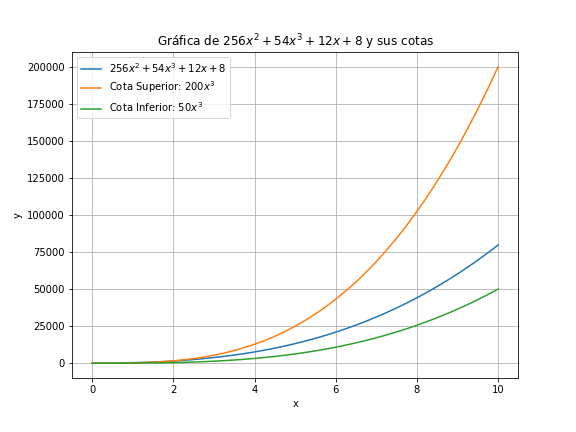
\includegraphics[width=14cm]{graph_1.png}
        \caption{Gráfica de  $256x^{2} + 54x^{3} + 12x + 8$ y un par de cotas}
        \label{fig:enter-label}
    \end{figure}
    
    
    \item \textbf{Dado un arreglo $A$ que tiene $n$ enteros $A_1, A_2, ..., A_n$, generar una matriz $B$ de $n$ por $n$ en donde $B_{ij}$ (para $i \leq j$) contiene la suma de los números del arreglo $A$, desde $A_i$ hasta $A_j$ $(A_i+A_{i+1}+...+A_{j})$. Los valores de $B_{ij} = 0$ para $i > j$. Un algoritmo simple para resolver el problema sería como el dado en el Algoritmo 1.}
    \begin{enumerate}
        \item \textbf{Dar un límite de forma $O(f(n))$ para el tiempo de ejecución del Algoritmo 1 y para una entrada de $n$ elementos. (\textbf{10 puntos})}

        A continuación se muestra un análisis visual del tiempo de ejecución que, dependiente de la entrada tomará $n$ ciclos de reloj ejecutar.

        \begin{figure}[H]
            \centering
            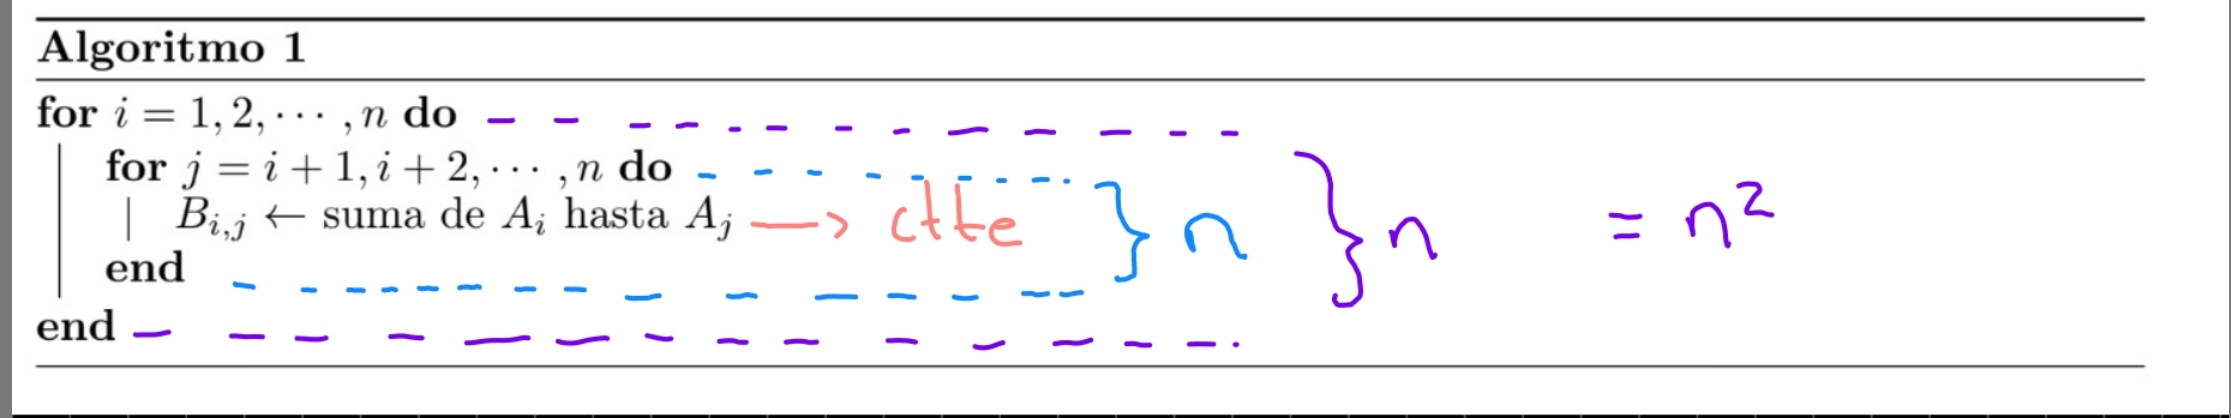
\includegraphics[width=16cm]{img_2.jpg}
            \caption{Análisis de algoritmo}
            \label{fig2}
        \end{figure}

        De tal forma que $O(n^2) = O(f(n))$\\
        
        \item \textbf{Para la misma función $f$, demuestre que el tiempo de ejecución del algoritmo es también $\Omega(f(n))$ y que también es $\Theta(f(n))$. (\textbf{15 puntos})}\\

        De nuevo, retomando la definición de : \textit{$f(n)$ pertenece a $\Omega(g(n))$ si existen las constantes positivas $n_0 \geq 0$ y $\epsilon > 0$ tal que para toda $n\geq n_0$ tenemos que $f(n) \geq \epsilon \cdot g(n)$}. Esto es: \\

        Si consideramos a $\epsilon$ = 1, entonces para toda $n \geq n_0$, para $n^2$, la igualdad $f(n) \geq \epsilon \cdot g(n)$ se cumple tal que $$n^2 \geq (1)\cdot n^2$$

        Con lo cual demostramos que $n^2 = \Omega(f(n))$. A su vez, al recordar que si $f(n) = O(f(n)) = \Omega(f(n))$, entonces también es verdad que $f(n) = \Theta(f(n))$, es decir es una cota estrecha. 
            
        \item \textbf{Dar un algoritmo alternativo para resolver el problema, que tenga un mejor tiempo de ejecución $O(g(n))$, donde $lim_{n \xrightarrow{}\infty} \frac{g(n)}{f(n)} = 0$. Demuéstrelo. (\textbf{25 puntos})}\\

        Por la naturaleza del problema, \textbf{no es posible encontrar una solución más eficiente}, pues para llenar una matriz de nxn elementos, se requiere forzosamente visitar cada elemento de la matríz para asignarle un valor, esto hace que siempre se requiere n*n ciclos de reloj, lo cual nos llevará a un tiempo de ejecución $O(n^2)$
        
        Para demostrar que no es posible encontrar un algoritmo más eficiente que \( O(n^2) \) para llenar una matriz de tamaño \( n \times n \),supongamos que tenemos una matriz \( M \) de tamaño \( n \times n \) que queremos llenar con valores constantes.
        
        Para llenar la matriz usando un algoritmo más eficiente que \( O(n^2) \), tendríamos que llenar todos los elementos en un tiempo inferior o al menos constante. Sin embargo, dado que la matriz tiene \( n^2 \) elementos, el tiempo total para llenar la matriz sería inferior a \( O(n^2) \).
        
        Esto contradice el hecho de que la matriz tiene \( n^2 \) elementos.
    
    \end{enumerate}

    
    \item \textbf{Dado el grafo de la Figura \ref{fig3}, demuestre que:}
    \begin{enumerate}
        \item \textbf{la arista $(a,b)$ no puede estar en el MST. (\textbf{10 puntos})}\\
        \begin{enumerate}
            \item  Dada la propiedad de ciclo, consideremos el ciclo formado por el subconjunto de nodos \{a,b,c\}.
            \item Supongamos que la arista $(a, b)$ pertenece al MST.

            \item Si borramos a la arista $(a, b)$, se genera un corte S en el MST, de forma que el conjunto de corte nuevo, contiene a las arista $(c,b)$ y $(c,a)$.

            \item Sin embargo, la arista f se encuentra tanto en el ciclo \{a,b,c\}
            , como en el conjunto de corte del corte S. Si fuera cierto que f pertenece al MST, entonces no debería existir otra arista que conecte al corte D, sin embargo existe otra arista que se encuentra en el ciclo \{a,b,c\} y en el conjunto de corte. Que es la arista $(c,a )$.

            \item Entonces, si el MST que no contiene a f tiene una arista en el conjunto de corte, con un peso menor, existirá entonces un MST llamado \textbf{T}. sin contener a f con un peso menor al MST que contiene a f. 

            \item Por lo tanto f no pertenece al MST.
        \end{enumerate}

        Una forma mas concisa de demostrarlo, es refiriéndonos directamente a la definición de la propiedad de ciclo, es decir, que dado el ciclo ciclo \{a,b,c\}, la arista de mayor costo en el ciclo no pertenece al MST. De esta forma es fácil ver que la arista $(a,b)$ no pertenece al MST
        
        \item \textbf{la arista $(c,f)$ debe estar en el MST. (\textbf{10 puntos})}
        \begin{enumerate}
            \item Dado que no existe la arista $(c,f)$, no es posible que exista dentro del MST.
            \item Sin embargo, si proponemos a la arista $(c,f)$ como una arista con un peso $w = \infty$, podemos realizar el análisis mediante la propiedad de ciclo similar al caso anterior.
            \item Al considerar el ciclo $\{a,c,f,d\}$, la arista $(c,f)$ sería la arista de mayor costo del ciclo y por lo tanto no pertenece al MST
            
        \end{enumerate}
        
    \end{enumerate}
    
    
    \item \textbf{Determine si el grafo de la Figura \ref{fig4} es bipartita. Fundamente su respuesta. (\textbf{20 puntos})}

    Dada la propiedad de que los grafos bipartitos no pueden tener ciclos de longitud impar, bastará con encontrar un ciclo de longitud impar para demostrar que no se trata de un grafo bipartito. 
    Como se puede observar en la Figura \ref{fig5}

    \begin{figure}[H]
    \centering
    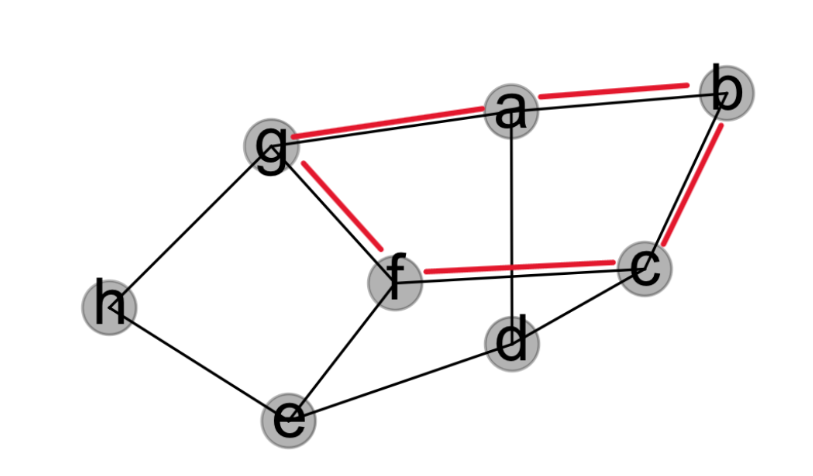
\includegraphics[width=10cm]{grafo_impart.png}
    \caption{ciclo impar en el Grafo 2 }
    \label{fig5}
\end{figure}

    \item \textbf{Escriba todos los órdenes topológicos del grafo de la Figura \ref{fig5}. (\textbf{15 puntos})}
    \begin{center}
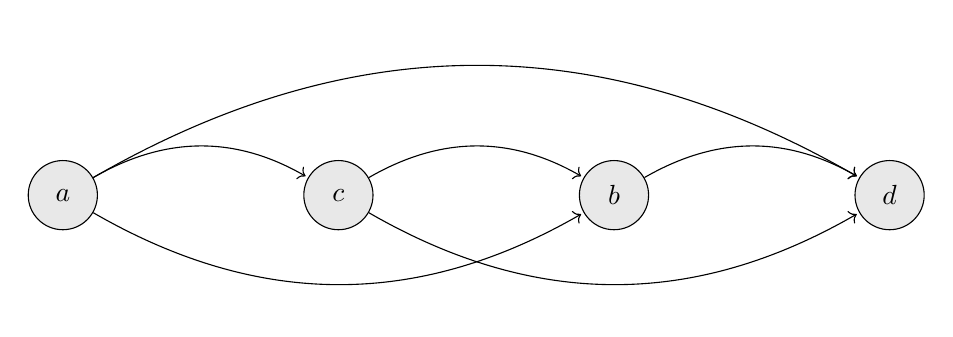
\begin{tikzpicture}[shorten >=1pt,node distance=3.5cm,on grid,auto]
  \tikzstyle{every state}=[fill={rgb:black,1;white,10}]

    \node[state] (a)                   {$a$};
    \node[state] (c)  [right of=a]    {$c$};
    \node[state] (b)  [right of=c]    {$b$};
    \node[state] (d)  [right of=b]    {$d$};
    
    \path[->]
    (a) edge [bend right]  node {}    (b)
    (a) edge [bend left]  node {}    (c)
    (a) edge [bend left]  node {}    (d)
    (b) edge [bend left]  node {}    (d)
    (c) edge [bend left]  node {}    (b)
    (c) edge [bend right]  node {}    (d)
    ;


\end{tikzpicture}
\end{center}

    
\end{enumerate}

\begin{figure}[H]
    \centering
    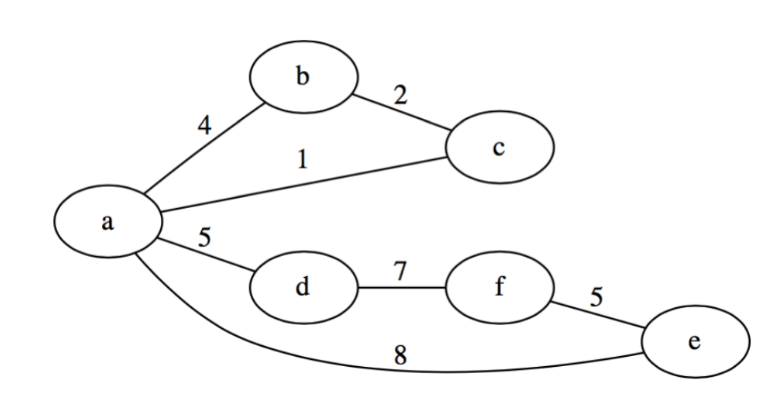
\includegraphics[width=10cm]{grafo_1.png}
    \caption{Grafo 1}
    \label{fig3}
\end{figure}

\begin{figure}[H]
    \centering
    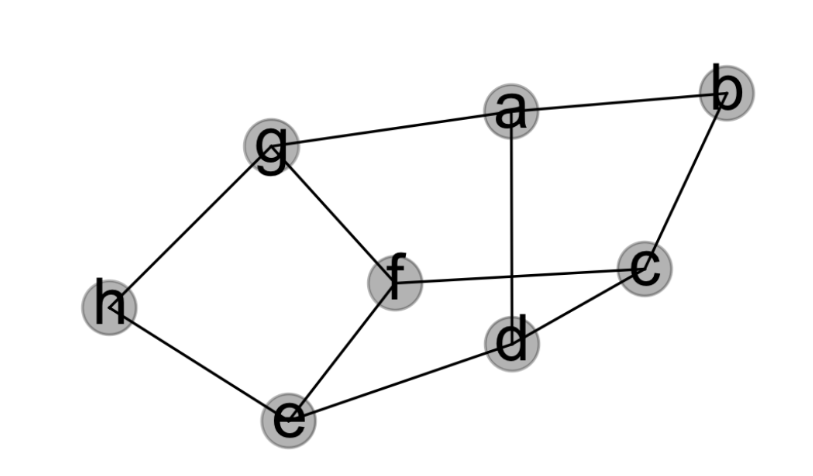
\includegraphics[width=10cm]{grafo_2.png}
    \caption{Grafo 2}
    \label{fig4}
\end{figure}


\begin{figure}[H]
    \centering
    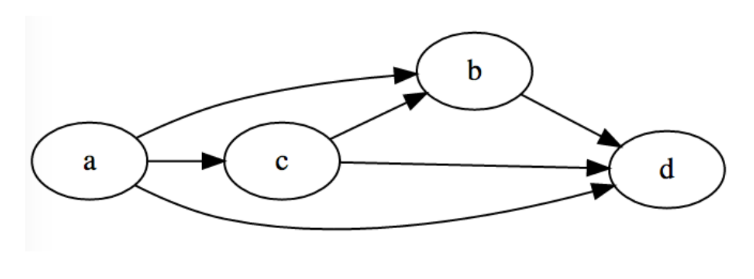
\includegraphics[width=10cm]{grafo_3.png}
    \caption{Grafo 3}
    \label{fig5}
\end{figure}


\end{document}
